
\begin{figure}[!ht]
  \hspace{28pt}
  \subfloat[]{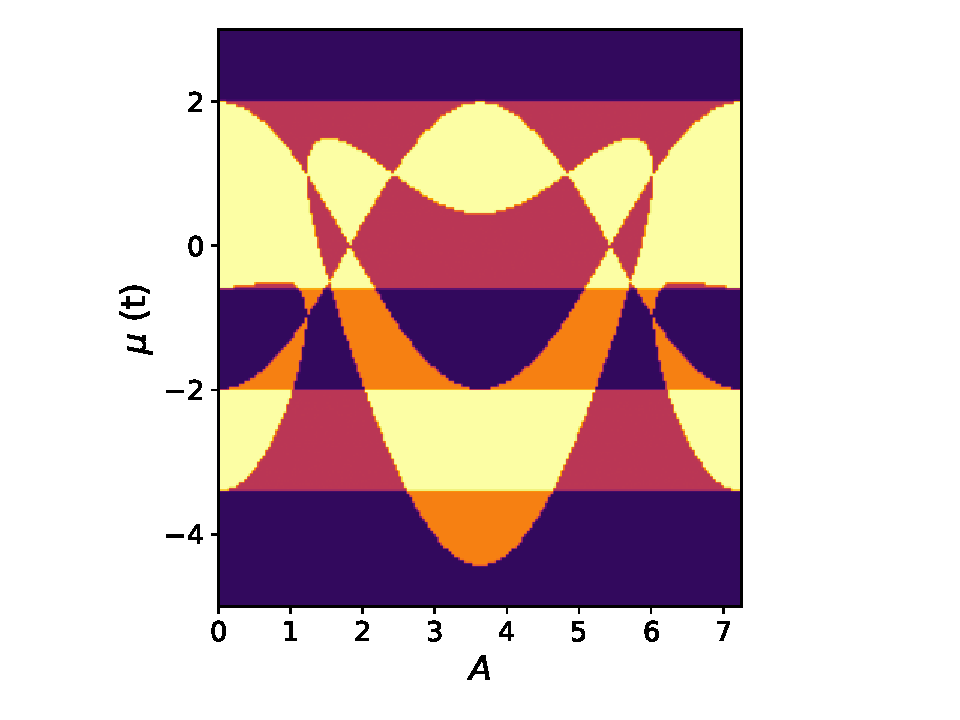
\includegraphics[width=0.50\textwidth]{./figures/supp/topological-phase-diagram-1pi6-n-3.pdf}}
  \hspace{-40pt}
  \subfloat[]{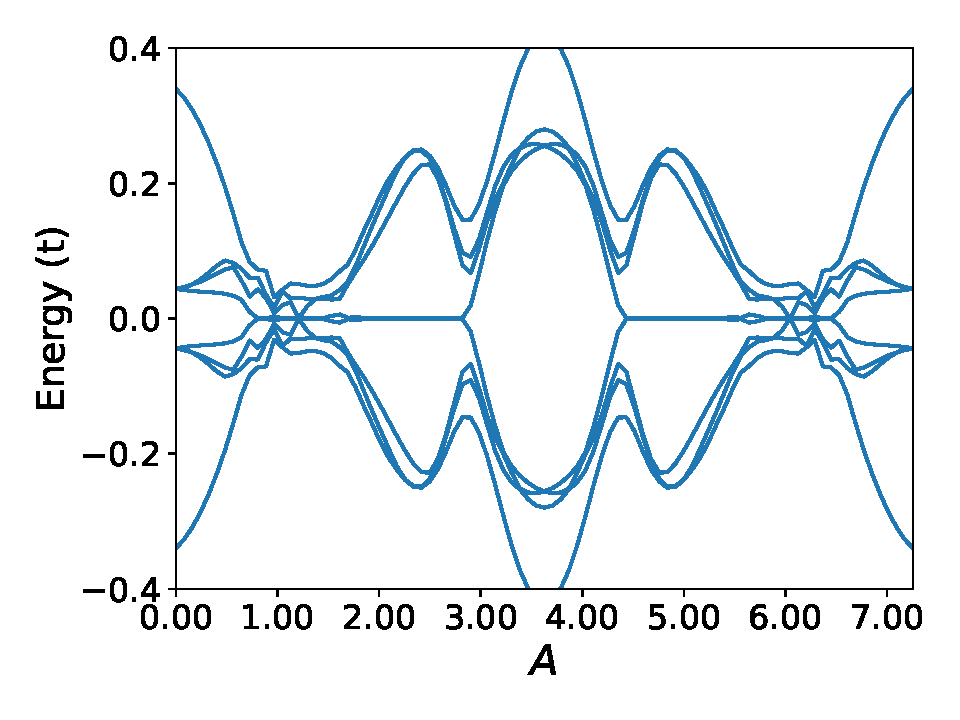
\includegraphics[width=0.50\textwidth]{./figures/supp/spectral-flow-nr-50-w-3-mu-1_6.pdf}} \\
  \hspace{70pt}
  \subfloat[]{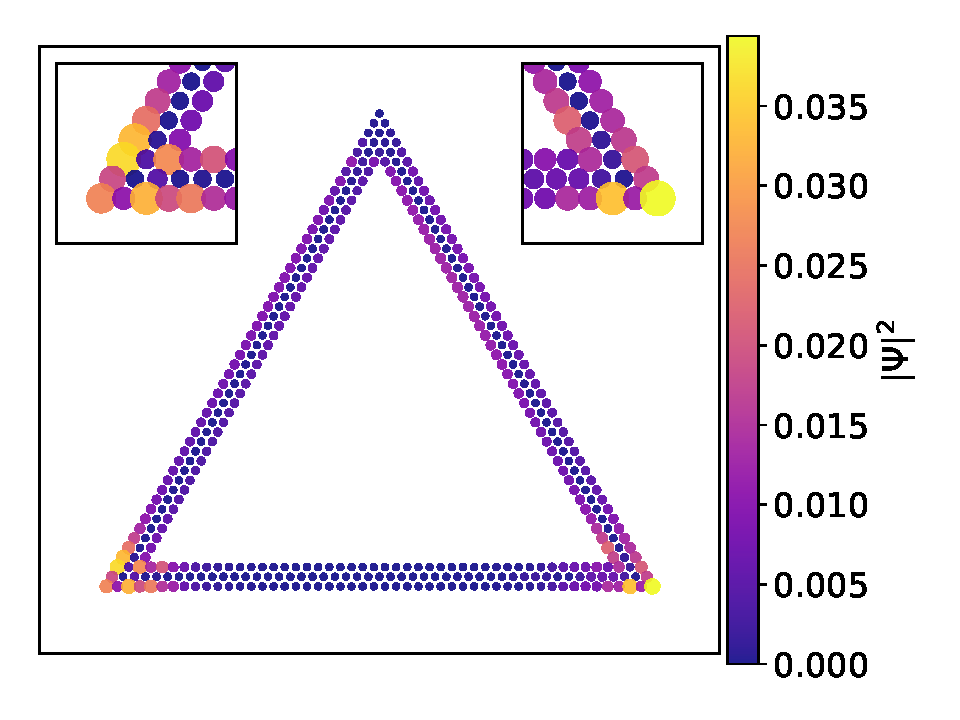
\includegraphics[width=0.50\textwidth]{./figures/supp/GS-A-2_74-nr-50-w-3-mu-1_6.pdf}}
  \caption{(a) Topological phase diagram for a $W=3$ hollow triangle obtained by overlapping the $\mathcal{M}(A, \mu)$ plots of 1D chains with $\mathbf A = A\hat{y}$ and $\mathbf A = A(\frac{\sqrt{      3}}{2}\hat{x}+\frac{1}{2}\hat{y})$. Color scheme: white---$\mathcal{M}=1$, dark blue---$\mathcal{M}=-1$, light blue---$\mathcal{M}=0$ (b) Near-gap BdG eigen-energies vs $A$ for a finite triangle with edge length $L=50$, $W=3$, and $\mu=1.6$. (c) BdG eigenfunction $|\Psi|^2$ summed over the two zero modes at $A=2.4709$.}
  \label{fig: supp pd}
\end{figure}

A model that is closer to a realistic hollow triangular island is the finite-width triangular chain or ribbon. An example, illustrated in Figure \ref{fig: supp pd} (c), has its edge length $L=50$ and width $W=3$. The phase diagram Fig.~\ref{fig: supp pd} (a) is created in a similar way as that in Fig. \ref{fig: pd} (a), assuming a constant vector potential and infinitely long $W=3$ ribbons. The spectral flow for the actual triangle with $\mu = 1.6$ in Fig.~\ref{fig: supp pd} (b) shows MZM in the parameter regions in agreement with the phase diagram. Fig.~\ref{fig: supp pd} (c) plots the MZM wavefunction for $A=2.7409$ and $\mu=1.6$ that are indeed well localized at the bottom corners.

\begin{figure}[!ht]
  \hspace{-20pt}
  \subfloat[]{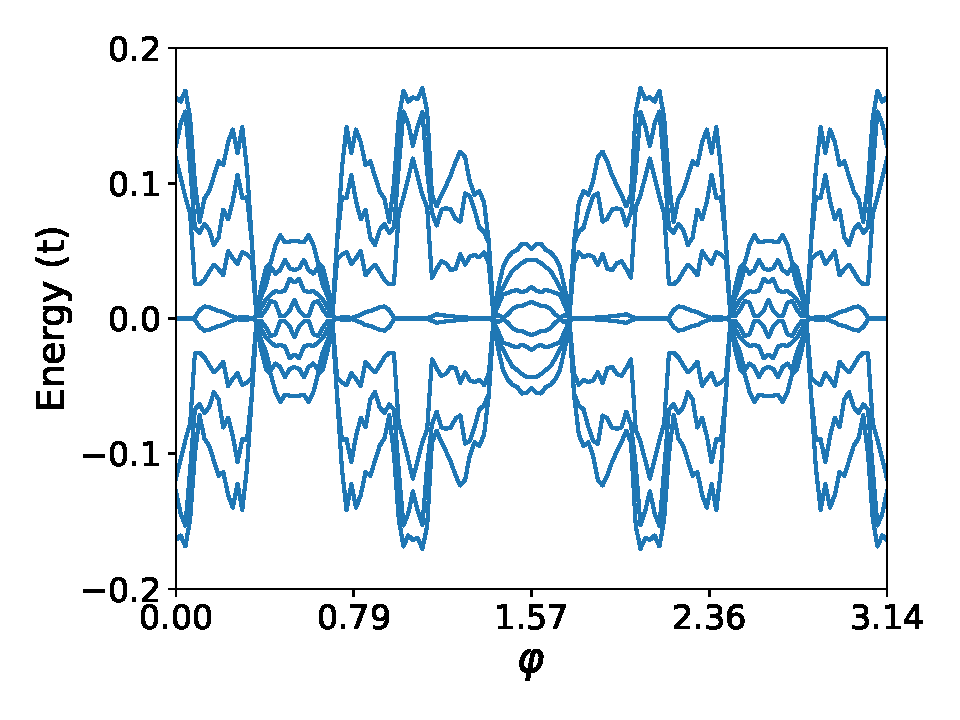
\includegraphics[width=0.5\textwidth]{./figures/supp/spectral-flow-w-3.pdf}}\\
  \subfloat[]{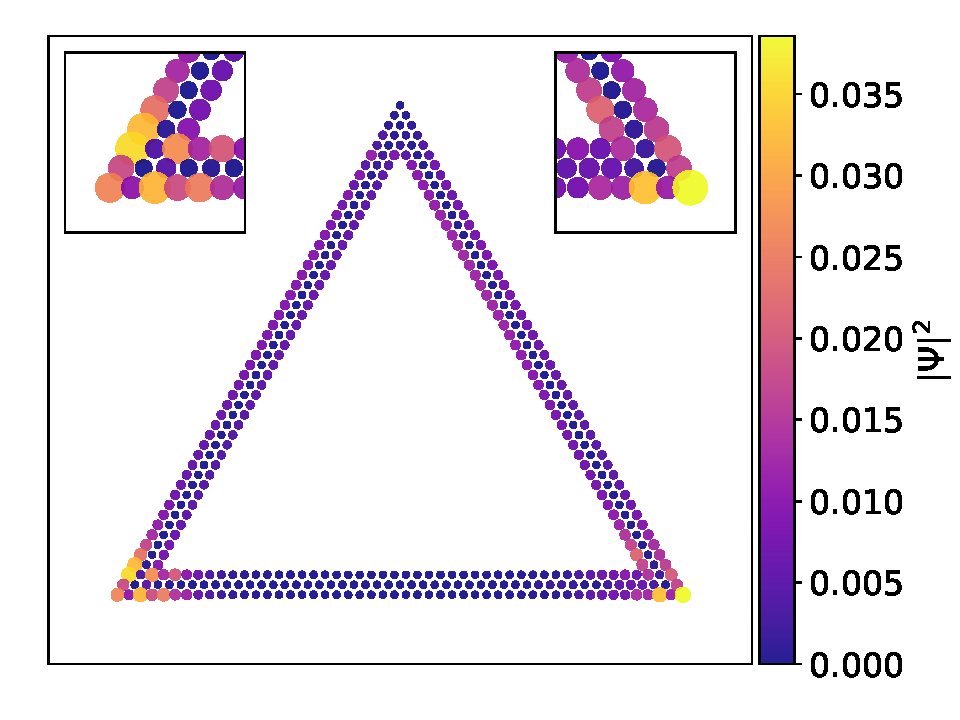
\includegraphics[width=0.4\textwidth]{./figures/supp/GS-T-Square-w-3.pdf}}
  %\subfloat[]{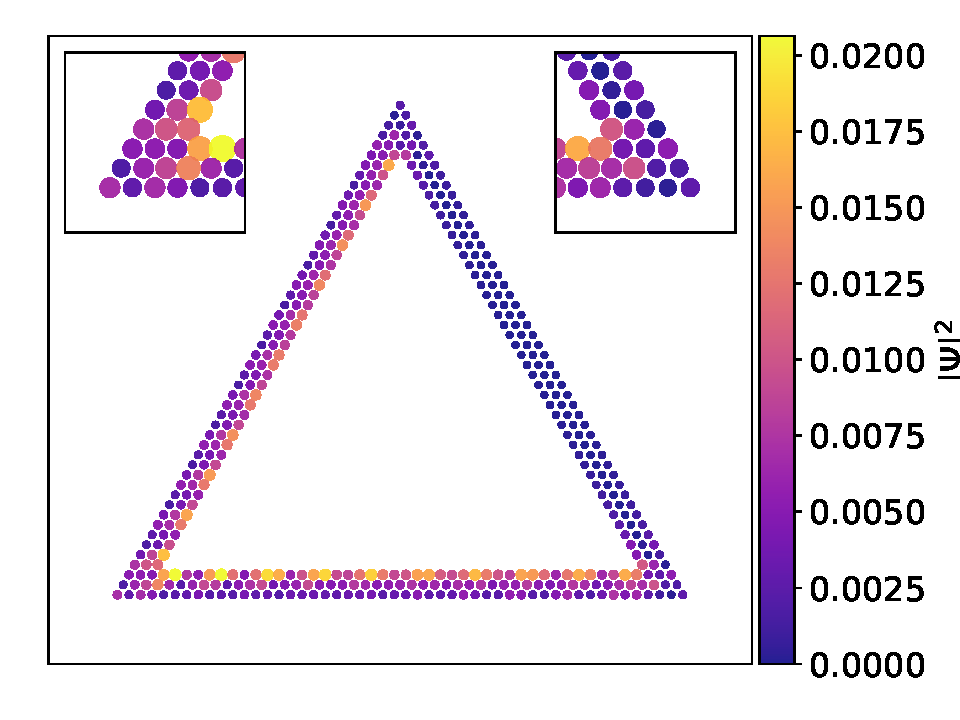
\includegraphics[width=0.4\textwidth]{./figures/supp/GS-T-Circle-w-3.pdf}}
  \subfloat[]{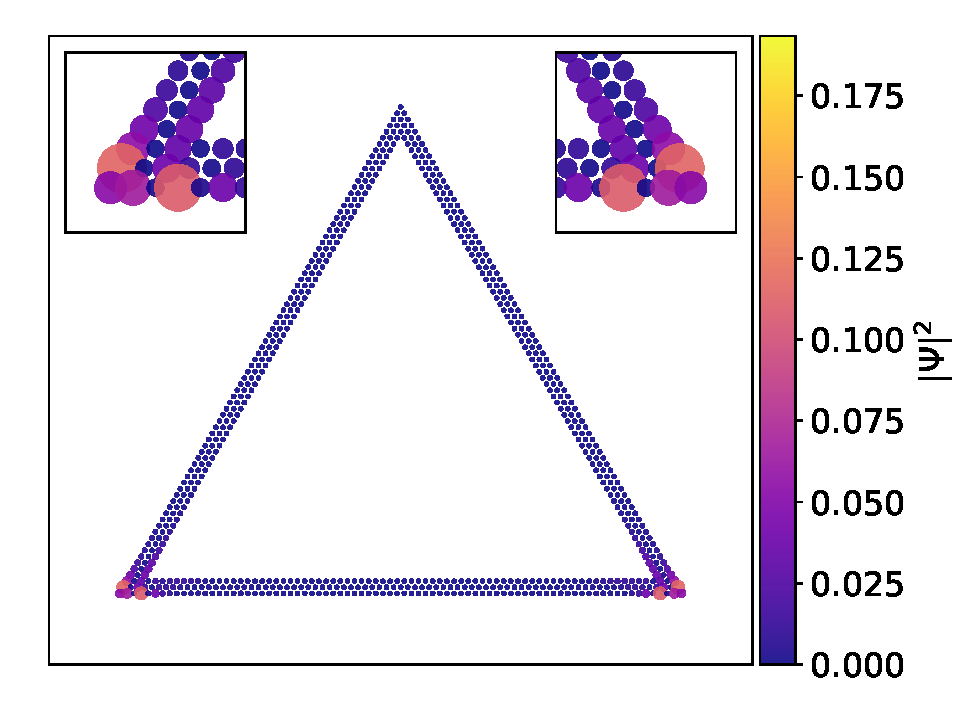
\includegraphics[width=0.4\textwidth]{./figures/supp/GS-T-Diamond-w-3.pdf}}
  \caption{(a) Spectral flow of a hollow triangle with $W=3$, $L=50$, $\mu=1.6$, and $A=2.75$ with increasing rotation angle $\varphi$, defined through $\mathbf A = A(-\sin\varphi \hat{x} + \cos\varphi \hat{y})$. (b-c) BdG eigenfunction $|\Psi|^2$ summed over the two zero modes at $\varphi = 0$ and $\frac{\pi}{3}$, respectively.}
  \label{fig: supp rotation}
\end{figure}

We next rotate the uniform vector potential to examine how the MZM move on a hollow triangle. Figure~\ref{fig: supp rotation} shows the spectral flow and eigenfunctions as we rotate $\varphi=0$ to $\varphi=\pi$ counterclockwisely. The two MZM cycle through the three vertices in a similar manner as that in Fig.~4 of the main text (only the MZM wavefunctions at $\varphi = 0$ and $\frac{\pi}{3}$ are plotted as representatives of the $\varphi = n\pi/3$ cases). Note that the spectral flow has 3-fold rotation symmetry but not 6-fold, since increasing $\varphi$ by $\frac{2\pi}{3}$ is equivalent to rotating the coordinate system clockwisely by $\frac{2\pi}{3}$. In contrast, rotating the vector potential by $\frac{\pi}{3}$, if without an additional sign change of the $p$-wave pairing potential, is not an exact symmetry of the finite triangle. Also we did not try to scrutinize the phase diagram to find a parameter path in which the bulk gap does not close, as in the $W=1$ case in the main text. Here we just point out that identifying a system-specific parameter path for adiabatic manipulation of MZM is in principle always possible, especially if one is allowed to have more knobs other than $\varphi$ in real structures, such as tuning the chemical potential of individual edges or the size of the vector potential, etc.

\section{Braiding MZM in a small network of triangles}

\begin{figure}[!ht]
  \hspace{-30pt}
  \subfloat[]{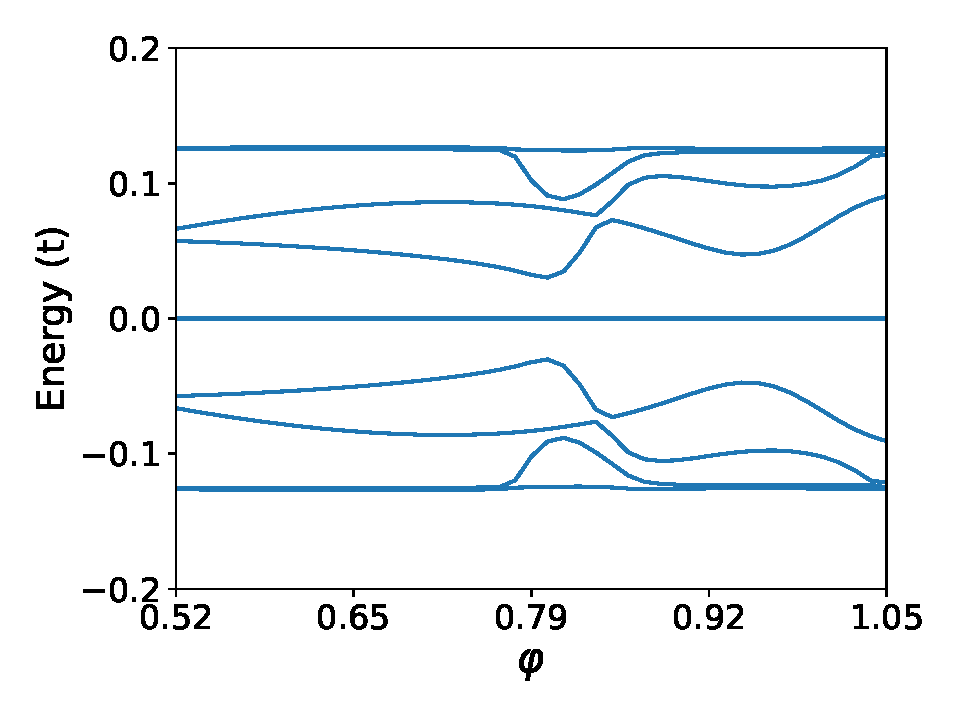
\includegraphics[width=0.4\textwidth]{./figures/supp/spectral-flow-braiding.pdf}} \\
  \vspace{-10pt}
  \subfloat[]{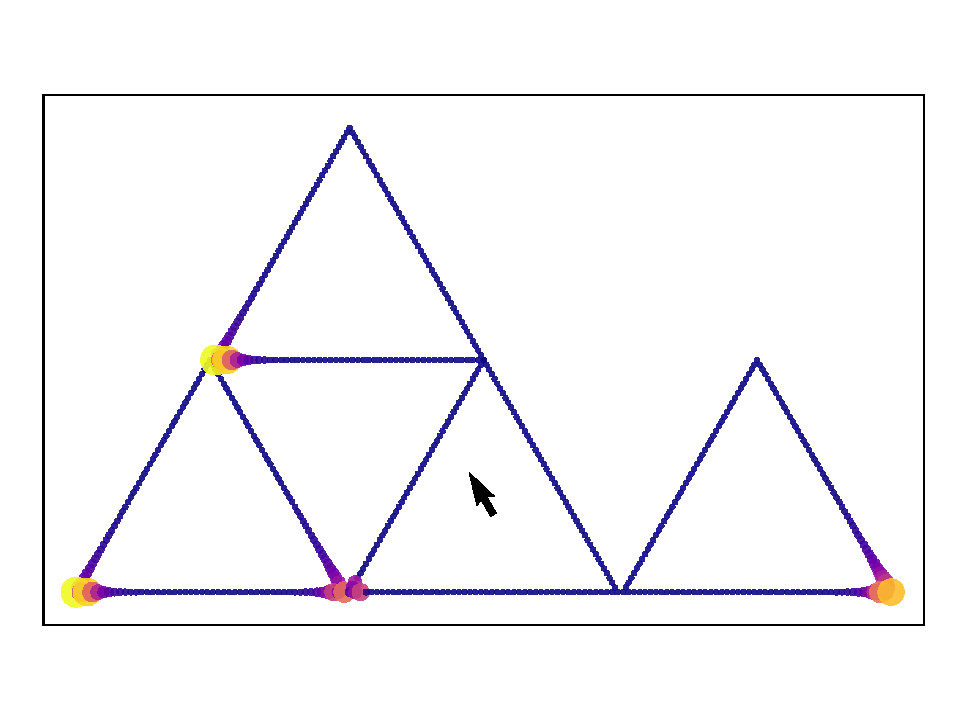
\includegraphics[width=0.30\textwidth]{./figures/supp/GS-T-0_5236.pdf}}
  \subfloat[]{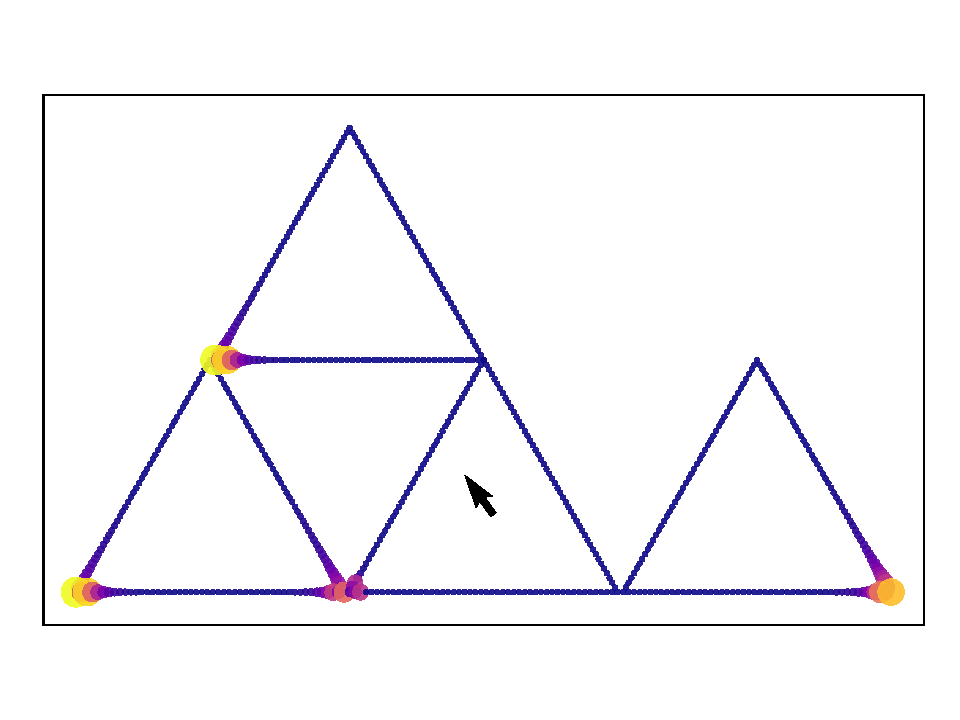
\includegraphics[width=0.30\textwidth]{./figures/supp/GS-T-0_6283.pdf}}
  \subfloat[]{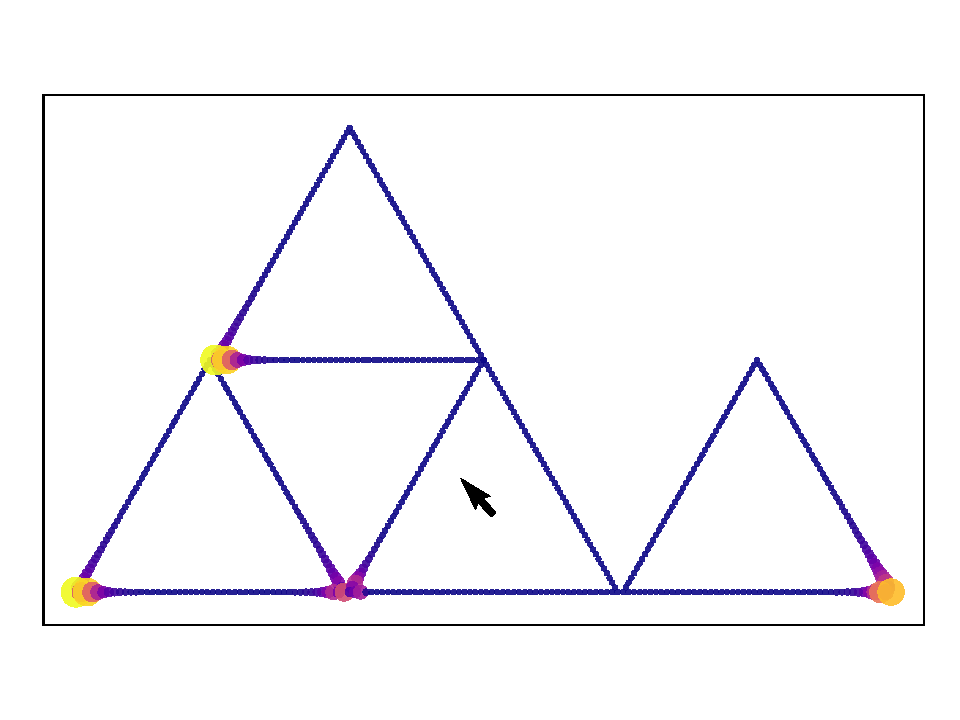
\includegraphics[width=0.30\textwidth]{./figures/supp/GS-T-0_7330.pdf}} \\
  \subfloat[]{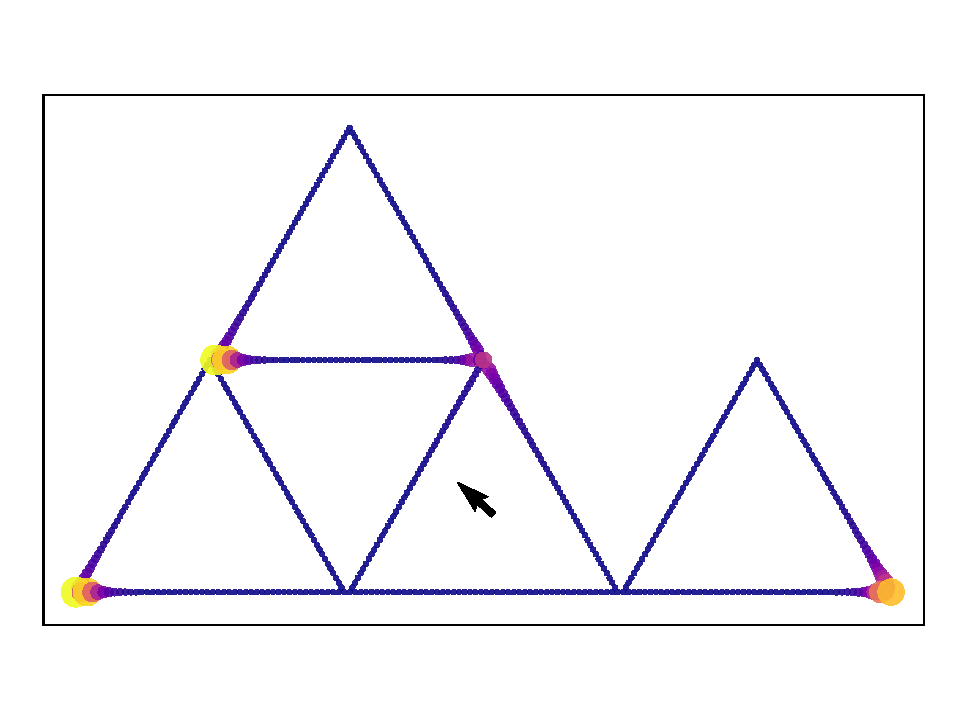
\includegraphics[width=0.30\textwidth]{./figures/supp/GS-T-0_8378.pdf}}
  \vspace{-10pt}
  \subfloat[]{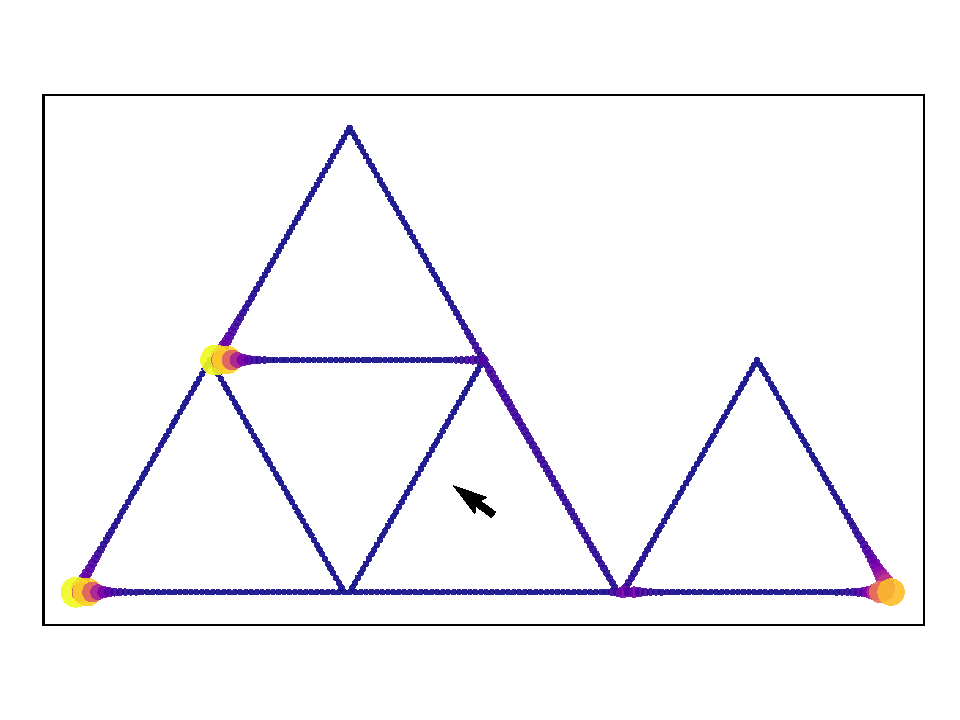
\includegraphics[width=0.30\textwidth]{./figures/supp/GS-T-0_9425.pdf}}
  \subfloat[]{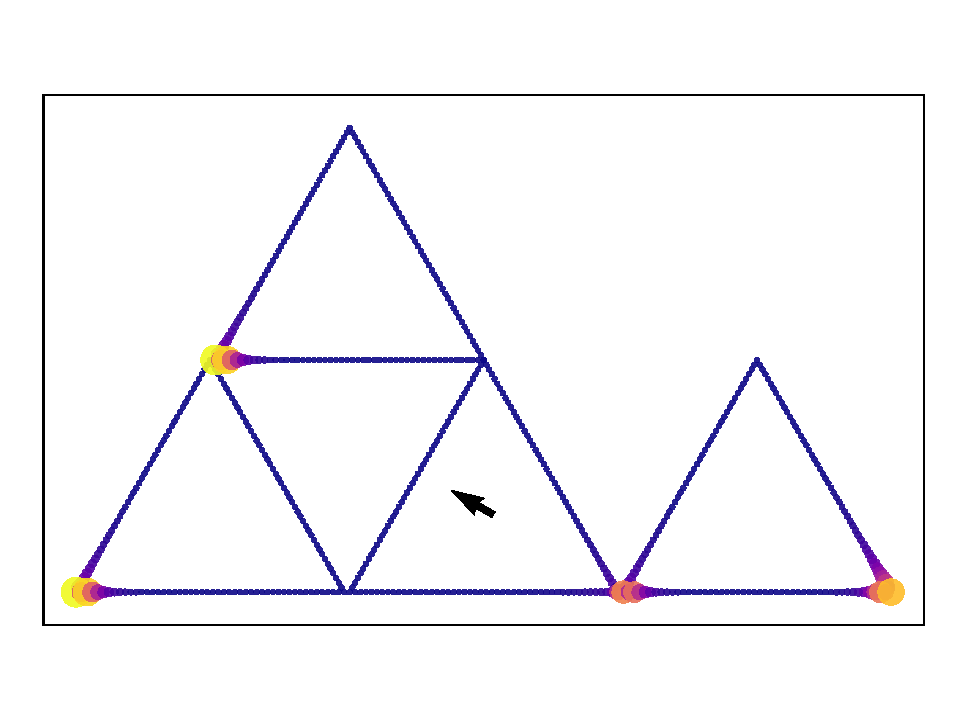
\includegraphics[width=0.30\textwidth]{./figures/supp/GS-T-1_0472.pdf}}
  \caption{(a) Spectral flow for the critical step of swapping $\gamma_2$ and $\gamma_3$ in the example of Fig.~5 in the main text, calculated using four corner-sharing triangles of $W=1$ and $L=50$, with $\mu=1.6$ and $A=2.6$. Vector potential for the middle triangle in the bottom row can rotate according to $\mathbf A = A(-\sin\varphi \hat{x} + \cos\varphi \hat{y})$ from $\varphi = \frac{\pi}{6}$ to $\frac{\pi}{3}$, while the other three have fixed $\varphi = 0$. (b)-(g) BdG eigenfunction $|\Psi|^2$ summed over the four zero modes at equally-spaced points along the rotation path. The black arrow indicates the direction of the vector potential for the bottom middle triangle.}\label{fig: supp braiding}
\end{figure}

In this section we show that one can braid two out of four MZM, a minimal setting for nontrivial manipulation of the degenerate many-body ground states, by using a small network of corner-sharing triangles. We focus on the critical step of swapping $\gamma_2$ and $\gamma_3$ as labeled in Fig.~5 of the main text. This can be done by rotating the vector potential of the triangle in the middle of the bottom row from $\varphi = \frac{\pi}{6}$ to $\frac{\pi}{3}$. More specifically, when $\varphi = \frac{\pi}{6}$, with the chosen values of $\mu$ and $A$, only the right edge of the said triangle is topologically nontrivial. The chain that hosts $\gamma_{3,4}$ thus extends through this nontrivial edge to the top triangle as in Fig.~\ref{fig: supp braiding} (b). On the other hand, when $\varphi$ increases to $\frac{\pi}{3}$, the nontrivial edge of the middle triangle changes from right to left, which leads to $\gamma_2$ hopping from its left corner to the right through the top corner, while $\gamma_3$ is unaffected [Figs.~\ref{fig: supp braiding} (c-g)]. As a result the $\gamma_2,\gamma_3$ swapping is done without closing the bulk gap, as can be seen from the spectral flow in Fig.~\ref{fig: supp braiding} (a).

